\subsection{Dot product}

\subsubsection{Implementation}
I compiled \texttt{Skeleton\_codes/dotProduct/dotProduct.cpp} with \texttt{g++ -fopenmp}. The Makefile exposes the vector size through the variable \texttt{N}, injected at compile time (``\texttt{-DN=\$(N)}''). The batch script \texttt{run\_jobs.sh} rebuilds the binary for each $N \in \{10^5,10^6,10^7,10^8\}$ and runs both OpenMP variants.

\lstinputlisting[
    caption={Reduction-based OpenMP dot product},
    captionpos=b,
    label={lst:dotprod_reduction},
    language=C++,
    numbers=left,
    linerange={57-67},
    firstnumber=57
]{../Skeleton_codes/dotProduct/dotProduct.cpp}

Listing~\ref{lst:dotprod_reduction} lets OpenMP handle partial sums via the \texttt{reduction} clause, avoiding explicit synchronisation. The alternative keeps thread-local buffers and merges them inside a \texttt{critical} region, shown in Listing~\ref{lst:dotprod_critical}.

\lstinputlisting[
    caption={Critical-based OpenMP dot product},
    captionpos=b,
    label={lst:dotprod_critical},
    language=C++,
    numbers=left,
    linerange={69-84},
    firstnumber=69
]{../Skeleton_codes/dotProduct/dotProduct.cpp}


\subsubsection{Testing}
For each size the script sweeps \texttt{OMP\_NUM\_THREADS} in $\{1,2,4,8,16,20\}$, exporting the value before invoking the executable. Each run stores its stdout to \texttt{logs/dotprod\_N\ldots\_T\ldots.log}; a Python helper converts the logs into the plots below and verifies that the reduction and critical versions match the serial dot product within a relative tolerance of $10^{-6}$.

\subsubsection{Discussion}
Figures~\ref{fig:dotprod_n1e5}--\ref{fig:dotprod_n1e8} show that even the smallest test ($N = 10^5$) benefits from parallelism: two threads reduce the runtime from $11.7\,\mathrm{ms}$ to $6.2\,\mathrm{ms}$ and eight threads reach $2.4\,\mathrm{ms}$. The efficiency plot in Figure~\ref{fig:dotprod_eff} highlights how OpenMP overhead grows with the thread count: efficiency is defined as $E = T_1 /(p \cdot T_p)$, so every time the speedup grows sub-linearly the per-core return decreases (e.g.\ speedup $\approx 2$ on two threads gives $E \approx 1$, speedup $\approx 4.9$ on eight threads gives $E \approx 0.6$). Beyond eight threads the serial portion and the \texttt{critical} synchronisation dominate, so efficiencies fall below $0.3$, even though the absolute runtime still drops (e.g.\ $T_{16} = 0.54\,\mathrm{s}$ for $N = 10^7$). The reduction variant consistently retains $5{-}10\%$ higher efficiency because it avoids serialised updates. Overall, multi-threading is worth, provided that the thread count remains modest (up to eight) to keep overhead under control for the smaller vectors; for $N \ge 10^7$ the reduction version scales well up to sixteen threads.

\begin{figure}[H]
    \centering
    \begin{subfigure}{0.45\textwidth}
        \centering
        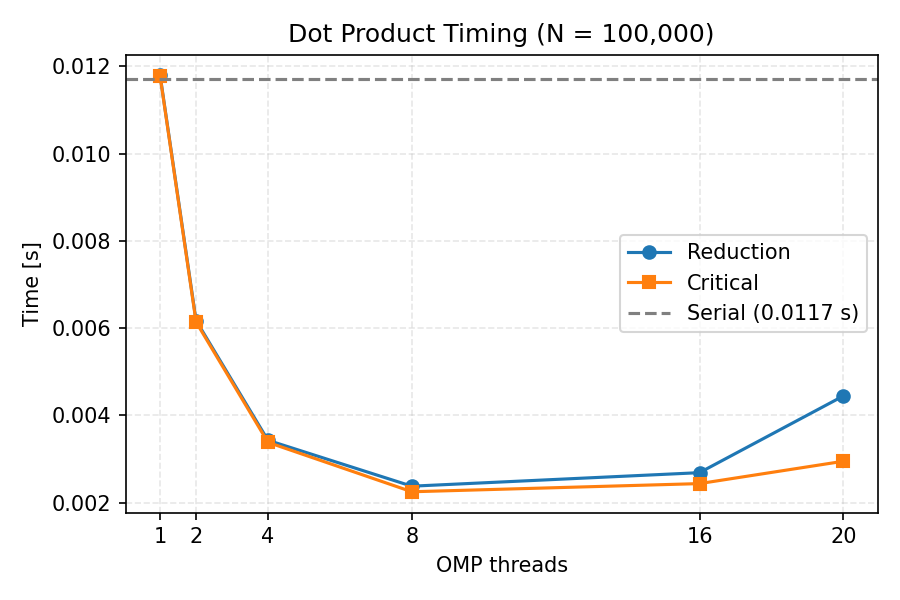
\includegraphics[width=\linewidth]{../Skeleton_codes/dotProduct/plots/dotprod_N100000.png}
        \caption{$N = 10^5$}
        \label{fig:dotprod_n1e5}
    \end{subfigure}
    \hfill
    \begin{subfigure}{0.45\textwidth}
        \centering
        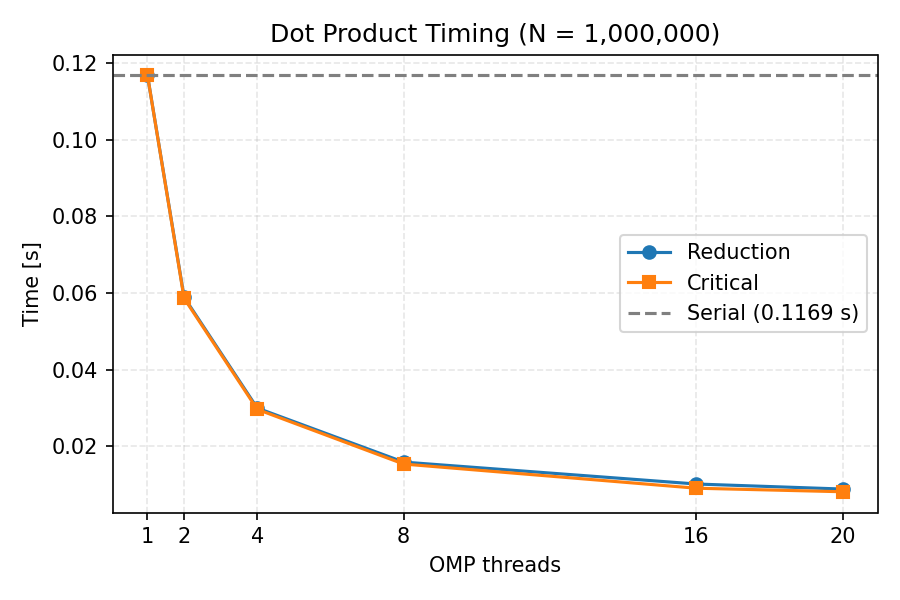
\includegraphics[width=\linewidth]{../Skeleton_codes/dotProduct/plots/dotprod_N1000000.png}
        \caption{$N = 10^6$}
        \label{fig:dotprod_n1e6}
    \end{subfigure}

    \vspace{1em}

    \begin{subfigure}{0.45\textwidth}
        \centering
        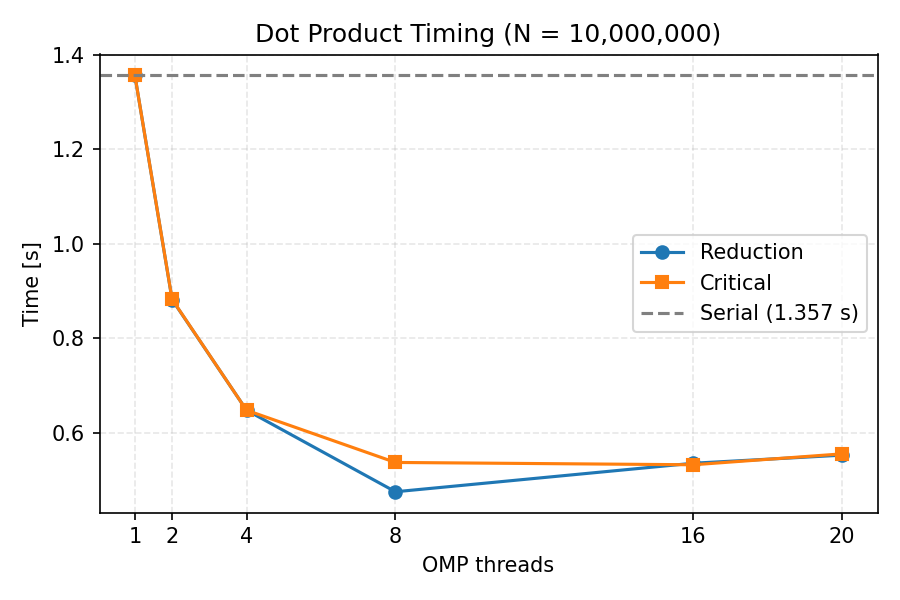
\includegraphics[width=\linewidth]{../Skeleton_codes/dotProduct/plots/dotprod_N10000000.png}
        \caption{$N = 10^7$}
        \label{fig:dotprod_n1e7}
    \end{subfigure}
    \hfill
    \begin{subfigure}{0.45\textwidth}
        \centering
        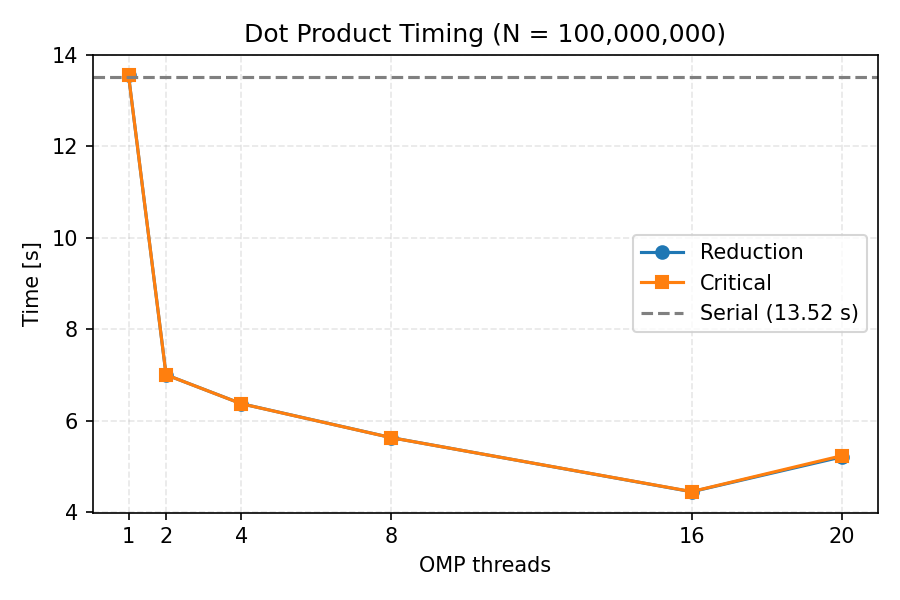
\includegraphics[width=\linewidth]{../Skeleton_codes/dotProduct/plots/dotprod_N100000000.png}
        \caption{$N = 10^8$}
        \label{fig:dotprod_n1e8}
    \end{subfigure}
    \caption{Execution time vs. threads for different vector sizes.}
\end{figure}

\begin{figure}[H]
    \centering
    \IfFileExists{../Skeleton_codes/dotProduct/plots/dotprod_efficiency.png}{
        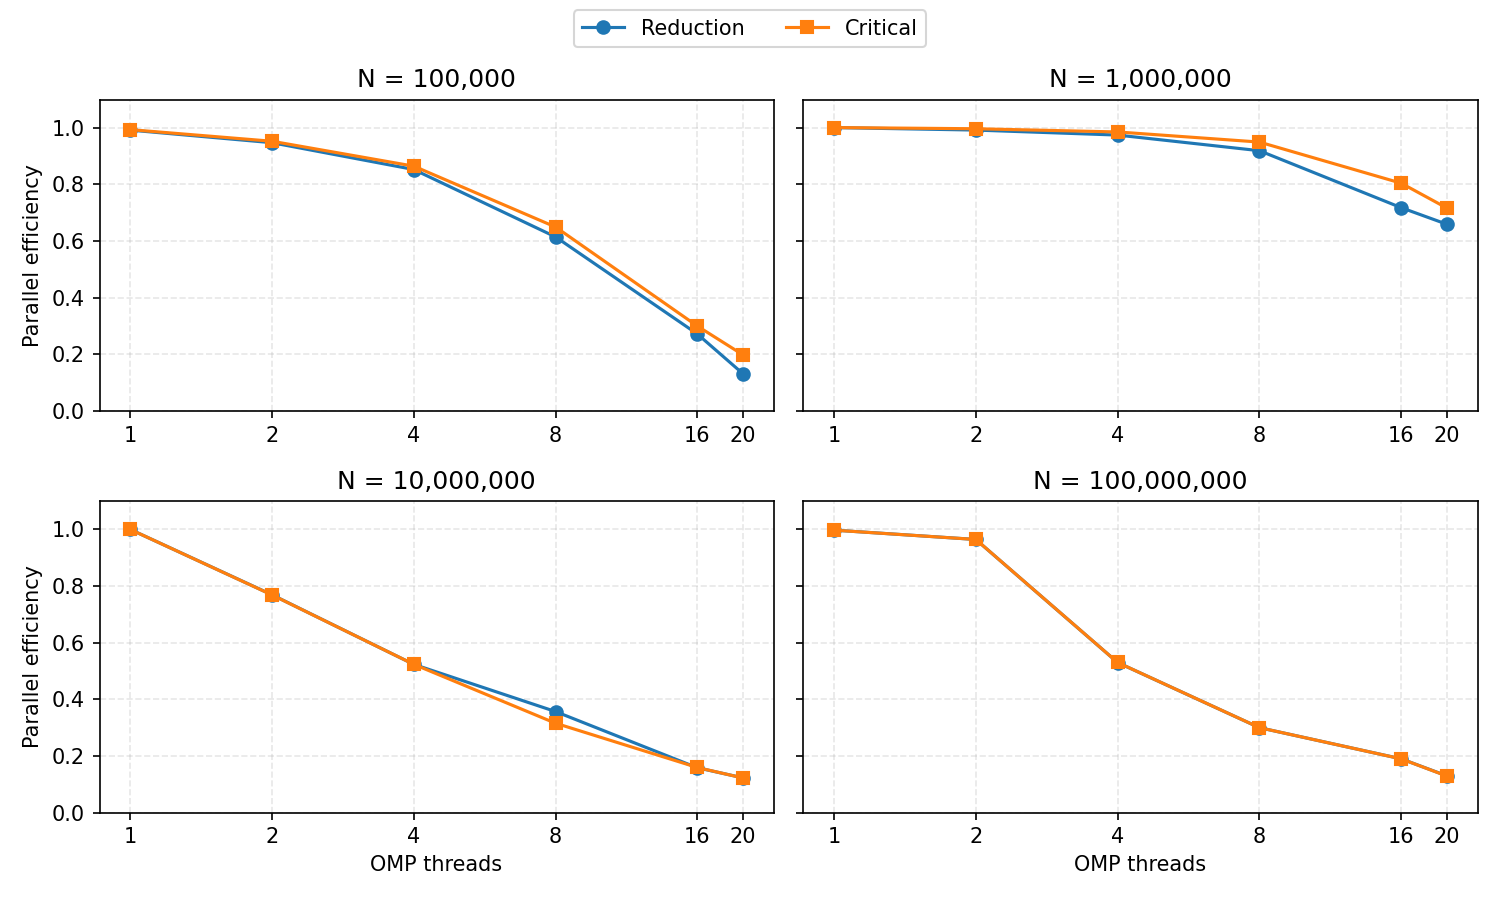
\includegraphics[width=0.75\linewidth]{../Skeleton_codes/dotProduct/plots/dotprod_efficiency.png}
    }{\fbox{Generate \texttt{dotprod\_efficiency.png} via \texttt{plot\_results.py}}}
    \caption{Parallel efficiency $E = T_1 / (p \cdot T_p)$ for the two OpenMP variants.}
    \label{fig:dotprod_eff}
\end{figure}




\subsection{Approximating $\pi$}

\subsubsection{Implementation}
I keep $N = 10^{10}$ as mandated. The serial loop in Listing~\ref{lst:pi_serial} walks through all indices with a single accumulator, while the OpenMP variant in Listing~\ref{lst:pi_parallel} retains the same structure but distributes iterations across threads using a reduction clause.

\lstinputlisting[
    caption={Serial midpoint integration for $\pi$},
    captionpos=b,
    label={lst:pi_serial},
    language=C++,
    numbers=left,
    linerange={18-25},
    firstnumber=18
]{../Skeleton_codes/pi/pi.cpp}

\lstinputlisting[
    caption={Parallel midpoint integration with OpenMP reduction},
    captionpos=b,
    label={lst:pi_parallel},
    language=C++,
    numbers=left,
    linerange={29-37},
    firstnumber=29
]{../Skeleton_codes/pi/pi.cpp}

The \texttt{reduction(+:\,sum)} clause is the natural choice here: it is an embarrassingly parallel loop, so each thread can integrate its chunk independently and OpenMP combines the private partial integrals at the end. This avoids serial bottlenecks (e.g., critical sections) and preserves the numerical result for the fixed $N = 10^{10}$.

\subsubsection{Results}

\begin{figure}[H]
    \IfFileExists{../Skeleton_codes/pi/plots/pi_speedup.csv}{
        \begin{subfigure}{0.45\textwidth}
            \centering
            \csvautotabular{../Skeleton_codes/pi/plots/pi_speedup.csv}
        \end{subfigure}
    }{\fbox{Generate \texttt{pi\_speedup.csv} via \texttt{plot\_speedup\_pi.py}}}
    \hfill
    \IfFileExists{../Skeleton_codes/pi/plots/pi_speedup.png}{
        \begin{subfigure}{0.45\textwidth}
            \centering
            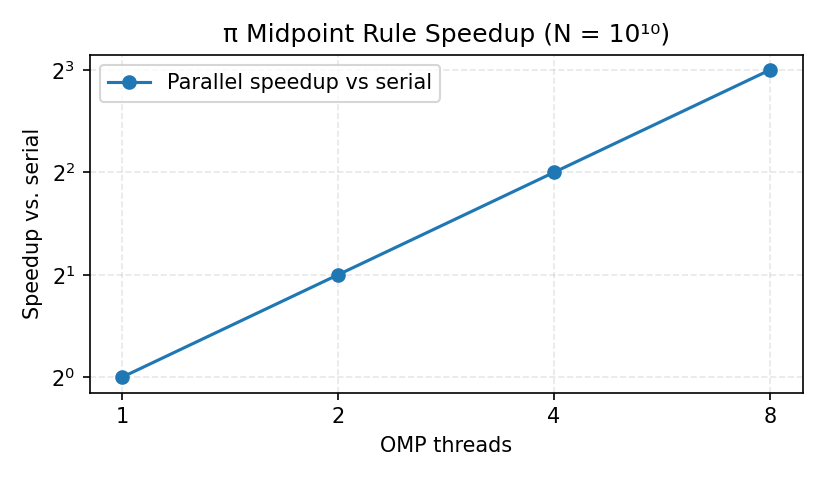
\includegraphics[width=\linewidth]{../Skeleton_codes/pi/plots/pi_speedup.png}
            \vspace{-7em}
        \end{subfigure}
    }{\fbox{Generate \texttt{pi\_speedup.png} via \texttt{plot\_speedup\_pi.py}}}
    \vspace{2em}
    \caption{Timings and speedup for the midpoint $\pi$ approximation with $N = 10^{10}$ (left) parallel speedup vs. serial baseline (right).}
    \label{fig:pi_speedup}
\end{figure}

Speedup ($S_p = T_1/T_p$) captures strong scaling: how much faster the fixed workload runs as threads increase. In this kernel each time the number of cores doubles the runtime halves (Table~\ref{fig:pi_speedup}), so the parallel efficiency $E_p = S_p/p$ stays essentially at one (e.g., $E_8 \approx 0.9997$). The loop is embarrassingly parallel and the OpenMP reduction introduces negligible overhead, so the dominant costs are the per-iteration arithmetic and loop control, which scale linearly with thread count. This demonstrates that the midpoint integration benefits directly from more cores while maintaining accuracy for the prescribed $N = 10^{10}$; an additional efficiency plot is unnecessary because the near-perfect speedup already shows the tight link between strong scaling and efficiency here.
